Modify the Tabular TD(0) algorithm for estimating $v_\pi$, to estimate $q_\pi$. 
%
\begin{figure}[h!]
  \center
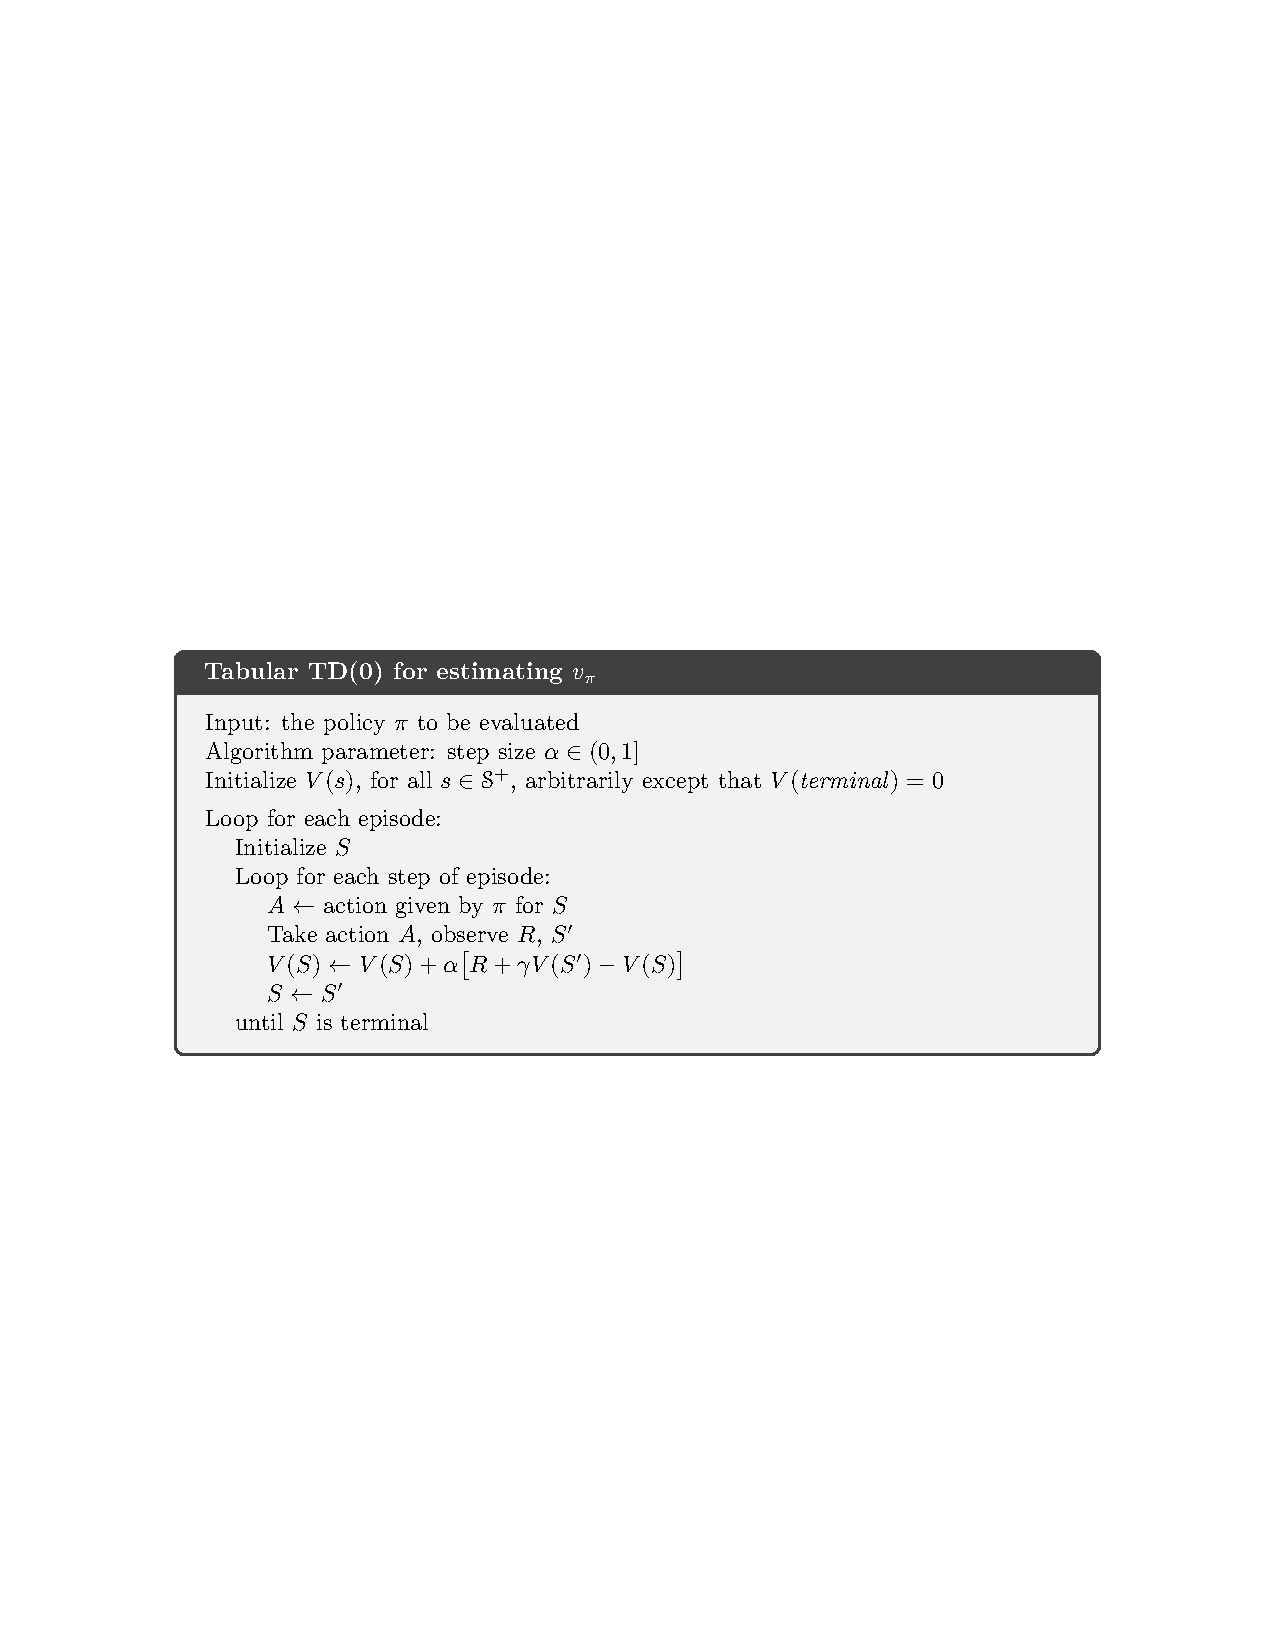
\includegraphics[width=0.85\linewidth]{figures/c2m2_td_alg.pdf}
\end{figure}

%% \textbf{Answer:}
%% \begin{tcolorbox}[title=Tabular TD(0) for estimating $q_\pi$]
%%   Input: the policy $\pi$ to be evaluated \\
%%   Algorithm parameter: step size $\alpha \in (0, 1]$ \\
%%     Initialize $Q(s, a)$, for all $s \in \mathcal{S}^+$, $a \in \mathcal{A}(s)$, arbitrarily except that $Q(terminal, \cdot) = 0$ \\ \\
%%     Loop for each episode: \\
%%     \phantom{---} Initialize $S$ \\
%%     \phantom{---} Choose action $A$ given by $\pi$ for $S$ \\
%%     \phantom{---} Loop for each step of episode \\ 
%%     \phantom{---} \phantom{---} Take action $A$, observe $R, S'$ \\
%%     \phantom{---} \phantom{---} Choose action $A'$ given by $\pi$ for $S'$ \\
%%     \phantom{---} \phantom{---} $Q(S, A) \leftarrow Q(S, A) + \alpha [R + \gamma Q(S', A') - Q(S, A)]$ \\ 
%%     \phantom{---} \phantom{---} $S \leftarrow S'; A \leftarrow A';$ \\
%%     \phantom{---} until $S$ is terminal. 
%% \end{tcolorbox}
